% Documents setup
\documentclass[french,11pt]{book}

% fix for pandoc 1.14
\providecommand{\tightlist}{%
  \setlength{\itemsep}{0pt}\setlength{\parskip}{0pt}}

\usepackage{tabu} % https://tex.stackexchange.com/questions/50332/vertical-spacing-of-a-table-cell

% Location of the csas-style repository: adjust path as needed
\newcommand{\locRepo}{csas-style}

% Use the style file in the csas-style repository (res-doc.sty)
\usepackage{\locRepo/res-doc-french}

% header-includes from R markdown entry


% Headers and footers
\lhead{}
% \lhead{}
\rhead{}
% \rfoot{DRAFT - DO NOT CITE}

%%%% Commands for title page etc %%%%%

% Publication year
\newcommand{\rdYear}{2021}

% Publication month
\newcommand{\rdMonth}{}

% Report number
\newcommand{\rdNumber}{8}

% Region
\newcommand{\rdRegion}{Pacific Region}

% Title
\newcommand{\rdTitle}{Évaluation des stratégies de rétablissement possibles pour le sébaste aux yeux jaunes (\emph{Sebastes ruberrimus}) des eaux intérieures de la Colombie-Britannique}

\newcommand{\rdISBN}{Fs70-5/2021-008F-PDF}
\newcommand{\rdCatNo}{978-0-660-38699-7}

% Author names separated by commas and ', and' for the last author in the format 'M.H. Grinnell' (use \textsuperscript{n} for addresses)
\newcommand{\rdAuth}{Dana R. Haggarty\textsuperscript{1}, Quang C. Huynh\textsuperscript{2}, Robyn E. Forrest\textsuperscript{1}, Sean C. Anderson\textsuperscript{1}, Midoli J. Bresch\textsuperscript{1}, Elise A. Keppel\textsuperscript{1}}

% Author names reversed separated by commas in the format 'Grinnell, M.H.'
\newcommand{\rdAuthRev}{Haggarty, D.R., C.R. Huynh, R.E. Forrest, S.C. Anderson, M.J. Bresch, et E.A. Keppel}

% Author addresses (use \textsuperscript{n})
\newcommand{\rdAuthAddy}{\textsuperscript{1}Station biologique du Pacifique\\
Pêches et Océans Canada, 3190, chemin Hammond Bay\\
Nanaimo (Colombie-Britannique) V9T 6N7, Canada\\

\textsuperscript{2}Institut pour les océans et la pêche\\
LRAE de l'Université de la Colombie- Britannique, 2202, Main Mall\\
Vancouver (Colombie-Britannique) V6T 1Z4, Canada\\}

\newcommand{\citationOtherLanguage}{Haggarty, D.R., Huynh, Q.C., Forrest, R.E., Anderson, S.C., Bresch, M.J., Keppel, E.A. 2021. Evaluation of potential rebuilding strategies for Inside Yelloweye Rockfish (\emph{Sebastes ruberrimus}) in British Columbia. DFO Can. Sci. Advis. Sec. Res. Doc. 2021/008. vi + 141 p.}

% Name of file with abstract and resume (see \abstract and \frenchabstract for requirements)
\newcommand{\rdAbstract}{\abstract{En vertu des politiques et de la législation canadiennes, il faut Eétablir un plan de rétablissement pour les stocks de poissons qui ont été évalués comme étant inférieurs au point de référence limite (PRL) afin de les ramener au-delà du PRL. Les plans de rétablissement doivent être fondés sur des objectifs caractérisés par 1) une cible, 2) un délai souhaité pour atteindre la cible et 3) une probabilité acceptable d'atteindre la cible. Les plans de rétablissement doivent également comprendre des mesures de gestion ou des procédures de gestion, des jalons cibles et être évalués régulièrement. \vspace{1.5mm} \break Le stock de sébaste aux yeux jaunes (\emph{Sebastes ruberrimus}) des eaux intérieures est un stock sur lequel on dispose de données limitées, présent dans la zone de gestion du poisson de fond 4B (détroit de la Reine-Charlotte, détroit de Georgie et détroit de Juan de Fuca) en Colombie-Britannique. Il a été évalué comme étant inférieur au PLR en 2010, ce qui a donné lieu à la publication d'un plan de rétablissement. Il est également inscrit en vertu de la \emph{Loi sur les espèces en péril} comme espèce préoccupante. L'actuelle procédure de gestion pour assurer le rétablissement est un total autorisé des captures (TAC) annuel fixe de 15 tonnes métriques, qui n'a pas été réévalué depuis la dernière évaluation. \vspace{1.5mm} \break Ce projet vise à fournir un avis scientifique à l'appui de la réévaluation du plan de rétablissement du sébaste aux yeux jaunes des eaux intérieures. Nous appliquons un nouveau cadre d'évaluation de la stratégie de gestion (le Cadre des procédures de gestion), récemment élaboré pour le poisson de fond de la Colombie-Britannique, afin d'évaluer le rendement des autres procédures de gestion à données limitées pour ce qui est de l'atteinte des objectifs de rétablissement. Le Cadre des procédures de gestion suit six étapes de pratiques exemplaires pour évaluer la stratégie de gestion~: 1) la définition du contexte décisionnel; 2) l'établissement des objectifs et des paramètres de rendement; 3) la précision des modèles opérationnels pour représenter le système sous-jacent et calculer les paramètres de rendement; 4) la sélection des procédures de gestion possibles; 5) la réalisation de simulations en boucle fermée afin d'évaluer le rendement des procédures de gestion; 6) la présentation des résultats pour faciliter l'évaluation des compromis. \vspace{1.5mm} \break Nous avons appliqué ce cadre pour évaluer le rendement de 34 procédures de gestion à données limitées pour ce qui est de l'atteinte de l'objectif principal, qui est de ramener le stock au-dessus du PRL sur 1,5 génération avec au moins une probabilité de réussite de 95 \% {[}19 fois sur 20{]}. Nous avons également évalué le rendement des procédures de gestion en ce qui concerne deux autres paramètres de conservation, quatre objectifs de prises moyennes et un objectif de variabilité des prises. Pour tenir compte de l'incertitude liée à la dynamique de la population sous-jacente et aux sources de données, nous avons élaboré six scénarios de modèles opérationnels de rechange, qui différaient de par les hypothèses précises du modèle et des données. Ces scénarios de modèles opérationnels ont été divisés en un « ensemble de référence » (quatre modèles opérationnels) et un « ensemble de robustesse » (deux modèles opérationnels). Nous avons conditionné tous les modèles opérationnels aux données sur les prises observées, aux indices de l'abondance et aux données accessibles sur la composition selon l'âge. Nous avons utilisé la simulation en boucle fermée pour évaluer le rendement des procédures de gestion et nous avons éliminé celles qui ne satisfaisaient pas à un ensemble de critères de base, ce qui a laissé cinq procédures de gestion possibles~: des procédures de gestion à prises constantes annuelles de 10 ou 15 tonnes et trois procédures de gestion qui ajustent le TAC en fonction de la pente relative de l'indice de l'abondance dans le relevé à la palangre sur fond dur dans les eaux intérieures. \vspace{1.5mm} \break Les cinq procédures de gestion finales atteignaient l'objectif principal avec une probabilité supérieure à 0,98 (49 fois sur 50), dans les scénarios des quatre modèles opérationnels de l'ensemble de référence, surtout qu'aucun des modèles opérationnels de l'ensemble de référence n'a estimé que le stock serait inférieur au PRL en 2020. Dans les scénarios des deux modèles opérationnels de l'ensemble de robustesse, le scénario qui simulait une plus grande variabilité dans le futur relevé à la palangre sur fond dur a donné des résultats semblables à ceux des scénarios de l'ensemble de référence. Cependant, dans le scénario qui supposait un taux de mortalité naturelle plus faible pour le stock (« M faible »), toutes les procédures de gestion avaient des probabilités plus basses d'atteindre l'objectif principal, la probabilité la plus faible étant atteinte par la procédure de gestion actuelle (prises constantes de 15 tonnes). \vspace{1.5mm} \break Nous présentons un certain nombre de visualisations pour illustrer les compromis entre les objectifs de conservation et de prises pour les différentes procédures de gestion dans d'autres scénarios de modèles opérationnels. Ces visualisations présentent les compromis sous forme de tableaux et de graphiques, destinés à faciliter le processus de sélection de la procédure de gestion finale. Étant donné que toutes les procédures de gestion ont atteint l'objectif principal dans les scénarios de l'ensemble de référence, il n'y avait pas de compromis important entre les objectifs de conservation et les objectifs de prises. Parmi les deux scénarios de l'ensemble de robustesse, les compromis étaient les plus évidents dans le scénario de M faible, où la probabilité d'atteindre l'objectif principal diminuait à mesure que la probabilité de prises moyennes à court terme de 10 tonnes augmentait. \vspace{1.5mm} \break Nous discutons des incertitudes majeures, y compris l'incertitude entourant la mortalité naturelle, la sélectivité et les prises historiques, en notant que nous avons tenté d'en tenir compte en évaluant le rendement des procédures de gestion dans plusieurs modèles opérationnels. Nous soulignons les problèmes concernant les estimations de l'état actuel du stock de sébaste aux yeux jaunes des eaux intérieures et le rôle des points de référence dans le Cadre des procédures de gestion. Nous formulons des recommandations sur la fréquence des évaluations et suggérons des déclencheurs pour la réévaluation. Nous évaluons également le rendement des procédures de gestion en ce qui concerne le respect de deux autres critères d'évaluation pour le Comité sur la situation des espèces en péril au Canada.}}

%%%% End of title page commands %%%%%

% \pdfcompresslevel=5 % faster PNGs

\setcounter{section}{0}

\bibliographystyle{csas-style/res-doc}

\usepackage{amsmath}
\usepackage{bm}

% commands and environments needed by pandoc snippets
% extracted from the output of `pandoc -s`
%% Make R markdown code chunks work
\usepackage{array}
\usepackage{amssymb,amsmath}
\usepackage{color}
\usepackage{fancyvrb}
% From default template:
\newcommand{\VerbBar}{|}
\newcommand{\VERB}{\Verb[commandchars=\\\{\}]}
\DefineVerbatimEnvironment{Highlighting}{Verbatim}{commandchars=\\\{\}}
% Add ',fontsize=\small' for more characters per line
\usepackage{framed}
\definecolor{shadecolor}{RGB}{248,248,248}
\newenvironment{Shaded}{\begin{snugshade}}{\end{snugshade}}
\newcommand{\AlertTok}[1]{\textcolor[rgb]{0.94,0.16,0.16}{#1}}
\newcommand{\AnnotationTok}[1]{\textcolor[rgb]{0.56,0.35,0.01}{\textbf{\textit{#1}}}}
\newcommand{\AttributeTok}[1]{\textcolor[rgb]{0.77,0.63,0.00}{#1}}
\newcommand{\BaseNTok}[1]{\textcolor[rgb]{0.00,0.00,0.81}{#1}}
\newcommand{\BuiltInTok}[1]{#1}
\newcommand{\CharTok}[1]{\textcolor[rgb]{0.31,0.60,0.02}{#1}}
\newcommand{\CommentTok}[1]{\textcolor[rgb]{0.56,0.35,0.01}{\textit{#1}}}
\newcommand{\CommentVarTok}[1]{\textcolor[rgb]{0.56,0.35,0.01}{\textbf{\textit{#1}}}}
\newcommand{\ConstantTok}[1]{\textcolor[rgb]{0.00,0.00,0.00}{#1}}
\newcommand{\ControlFlowTok}[1]{\textcolor[rgb]{0.13,0.29,0.53}{\textbf{#1}}}
\newcommand{\DataTypeTok}[1]{\textcolor[rgb]{0.13,0.29,0.53}{#1}}
\newcommand{\DecValTok}[1]{\textcolor[rgb]{0.00,0.00,0.81}{#1}}
\newcommand{\DocumentationTok}[1]{\textcolor[rgb]{0.56,0.35,0.01}{\textbf{\textit{#1}}}}
\newcommand{\ErrorTok}[1]{\textcolor[rgb]{0.64,0.00,0.00}{\textbf{#1}}}
\newcommand{\ExtensionTok}[1]{#1}
\newcommand{\FloatTok}[1]{\textcolor[rgb]{0.00,0.00,0.81}{#1}}
\newcommand{\FunctionTok}[1]{\textcolor[rgb]{0.00,0.00,0.00}{#1}}
\newcommand{\ImportTok}[1]{#1}
\newcommand{\InformationTok}[1]{\textcolor[rgb]{0.56,0.35,0.01}{\textbf{\textit{#1}}}}
\newcommand{\KeywordTok}[1]{\textcolor[rgb]{0.13,0.29,0.53}{\textbf{#1}}}
\newcommand{\NormalTok}[1]{#1}
\newcommand{\OperatorTok}[1]{\textcolor[rgb]{0.81,0.36,0.00}{\textbf{#1}}}
\newcommand{\OtherTok}[1]{\textcolor[rgb]{0.56,0.35,0.01}{#1}}
\newcommand{\PreprocessorTok}[1]{\textcolor[rgb]{0.56,0.35,0.01}{\textit{#1}}}
\newcommand{\RegionMarkerTok}[1]{#1}
\newcommand{\SpecialCharTok}[1]{\textcolor[rgb]{0.00,0.00,0.00}{#1}}
\newcommand{\SpecialStringTok}[1]{\textcolor[rgb]{0.31,0.60,0.02}{#1}}
\newcommand{\StringTok}[1]{\textcolor[rgb]{0.31,0.60,0.02}{#1}}
\newcommand{\VariableTok}[1]{\textcolor[rgb]{0.00,0.00,0.00}{#1}}
\newcommand{\VerbatimStringTok}[1]{\textcolor[rgb]{0.31,0.60,0.02}{#1}}
\newcommand{\WarningTok}[1]{\textcolor[rgb]{0.56,0.35,0.01}{\textbf{\textit{#1}}}}

\newcommand{\lt}{\ensuremath <}
\newcommand{\gt}{\ensuremath >}

%Defines cslreferences environment
%Required by pandoc 2.8
%Copied from https://github.com/rstudio/rmarkdown/issues/1649

\DeclareGraphicsExtensions{.png,.pdf}
\begin{document}
\renewcommand{\tablename}{Tableau}
\frontmatter

\clearpage

\hypertarget{sec:introduction}{%
\section{INTRODUCTION}\label{sec:introduction}}

Ce projet vise à fournir un avis scientifique à l'appui de la révision du plan de rétablissement du stock de sébaste aux yeux jaunes (\emph{Sebastes ruberrimus}) des eaux intérieures (DFO \protect\hyperlink{ref-ifmp2018}{2018}), conformément aux directives stratégiques nationales (DFO \protect\hyperlink{ref-dfo2009}{2009}, \protect\hyperlink{ref-dfo2013}{2013}). Il applique un cadre de simulation en boucle fermée (Anderson et al. \protect\hyperlink{ref-anderson2020gfmp}{2020}\protect\hyperlink{ref-anderson2020gfmp}{a}) pour évaluer le rendement des procédures de gestion de rechange en ce qui concerne les objectifs de rétablissement du stock de sébaste aux yeux jaunes des eaux intérieures.

\hypertarget{sec:introduction-motivation}{%
\subsection{MOTIVATION~: OBLIGATIONS STRATÉGIQUES ET LÉGISLATIVES}\label{sec:introduction-motivation}}

Le Cadre pour la pêche durable du Canada jette les bases de l'approche de précaution en matière de gestion des pêches au Canada (DFO \protect\hyperlink{ref-dfo2006}{2006}, \protect\hyperlink{ref-dfo2009}{2009}). Le Cadre de l'approche de précaution (DFO \protect\hyperlink{ref-dfo2009}{2009}) repose sur la définition des points de référence biologiques qui définissent les cibles de la biomasse ainsi que les seuils de biomasse faible à éviter avec une probabilité élevée. L'approche exige que la mortalité par pêche soit ajustée par rapport à deux niveaux de l'état des stocks~: un point de référence supérieur du stock (RSS) et un point de référence limite (PRL) (figure~\ref{fig:pa-illustration}). Le PRL et le RSS délimitent trois zones d'état des stocks (« critique », « de prudence » et « saine »). Il faut établir un plan de rétablissement pour les stocks de poissons canadiens qui ont été évalués comme étant inférieurs au PRL, c.-à-d.~dans la zone critique (DFO \protect\hyperlink{ref-dfo2009}{2009}), afin de les ramener au-dessus du PRL (DFO \protect\hyperlink{ref-dfo2013}{2013}).


\begin{figure}[htb]

{\centering \pdftooltip{\includegraphics[width=3.8in]{C:/GitHub/yelloweye-inside/figs-french/pa-framework}}{Figure \ref{fig:pa-illustration}} 

}

\caption{Illustration du Cadre de l'approche de précaution du MPO. D'après DFO (\protect\hyperlink{ref-dfo2009}{2009}).}\label{fig:pa-illustration}
\end{figure}
En juin 2019, d'importantes modifications apportées à la \emph{Loi sur les pêches} du Canada ont légiféré de nombreux éléments clés du Cadre pour la pêche durable, qui sont enchâssés dans les dispositions sur les stocks de poissons (\href{https://laws-lois.justice.gc.ca/fra/lois/f-14/page-3.html\#h-1175547}{article 6 de la \emph{Loi sur les pêches}}. Les dispositions relatives aux stocks de poissons exigent que les principaux stocks soient gérés à des niveaux durables, en particulier à des niveaux de biomasse supérieurs au PRL. De plus, le paragraphe 6.2(1) stipule que si un grand stock de poissons a diminué en deçà de son PRL, un plan de rétablissement doit être établi pour reconstituer le stock au-dessus du PRL. Les grands stocks de poissons seront désignés en vertu d'un règlement, le premier lot de stocks devant l'être à l'automne 2020.

En vertu des directives sur l'élaboration de plans de rétablissement au Canada (DFO \protect\hyperlink{ref-dfo2013}{2013}), les plans de rétablissement doivent être fondés sur des objectifs caractérisés par~:
\begin{enumerate}
\def\labelenumi{\arabic{enumi}.}

\item
  une cible;
\item
  un délai souhaité pour atteindre la cible;
\item
  une probabilité acceptable convenue d'atteindre la cible.
\end{enumerate}
Les plans de rétablissement doivent également comprendre des mesures de gestion planifiées (les procédures de gestion), des jalons cibles et leur rendement doit faire l'objet d'examens réguliers (tous les trois ans), en plus de la surveillance et de l'évaluation annuelles. Les directives actuelles indiquent que le délai de rétablissement doit être de 1,5 à 2 fois la durée de génération de l'espèce (DFO \protect\hyperlink{ref-dfo2013}{2013}), la durée de génération étant le nombre moyen d'années entre la naissance d'un individu et la naissance de sa progéniture.

\hypertarget{sec:introduction-background}{%
\subsection{CONTEXTE}\label{sec:introduction-background}}

Le sébaste aux yeux jaunes des eaux intérieures est présent dans la zone de gestion 4B du poisson de fond en Colombie-Britannique (Figure~\ref{fig:map-4B}). Il devrait être désigné comme grand stock de poissons à l'automne 2020, date à laquelle sa gestion sera légiférée en vertu des dispositions sur les stocks de poissons. Le stock a été évalué comme étant inférieur au PLR en 2010 (Yamanaka et al. \protect\hyperlink{ref-yamanaka2011}{2011}; DFO \protect\hyperlink{ref-dfo2012}{2012}). De ce fait, un plan de rétablissement a été élaboré et publié à l'annexe 9 du Plan de gestion intégrée des pêches de la région du Pacifique pour le poisson de fond (DFO \protect\hyperlink{ref-ifmp2018}{2018}). Le stock de sébaste aux yeux jaunes des eaux intérieures est également inscrit en vertu de la \emph{Loi sur les espèces en péril} (LEP) comme espèce préoccupante (COSEWIC \protect\hyperlink{ref-cosewic2008}{2008}) et il est prévu que le Comité sur la situation des espèces en péril au Canada (COSEPAC) le réévaluera en 2020. Les résultats de ce projet pourraient guider la réévaluation du COSEPAC et, éventuellement, une évaluation du potentiel de rétablissement en vertu de la LEP, s'il y a lieu (voir l'annexe~\ref{app:cosewic}).


\begin{figure}[htb]

{\centering \pdftooltip{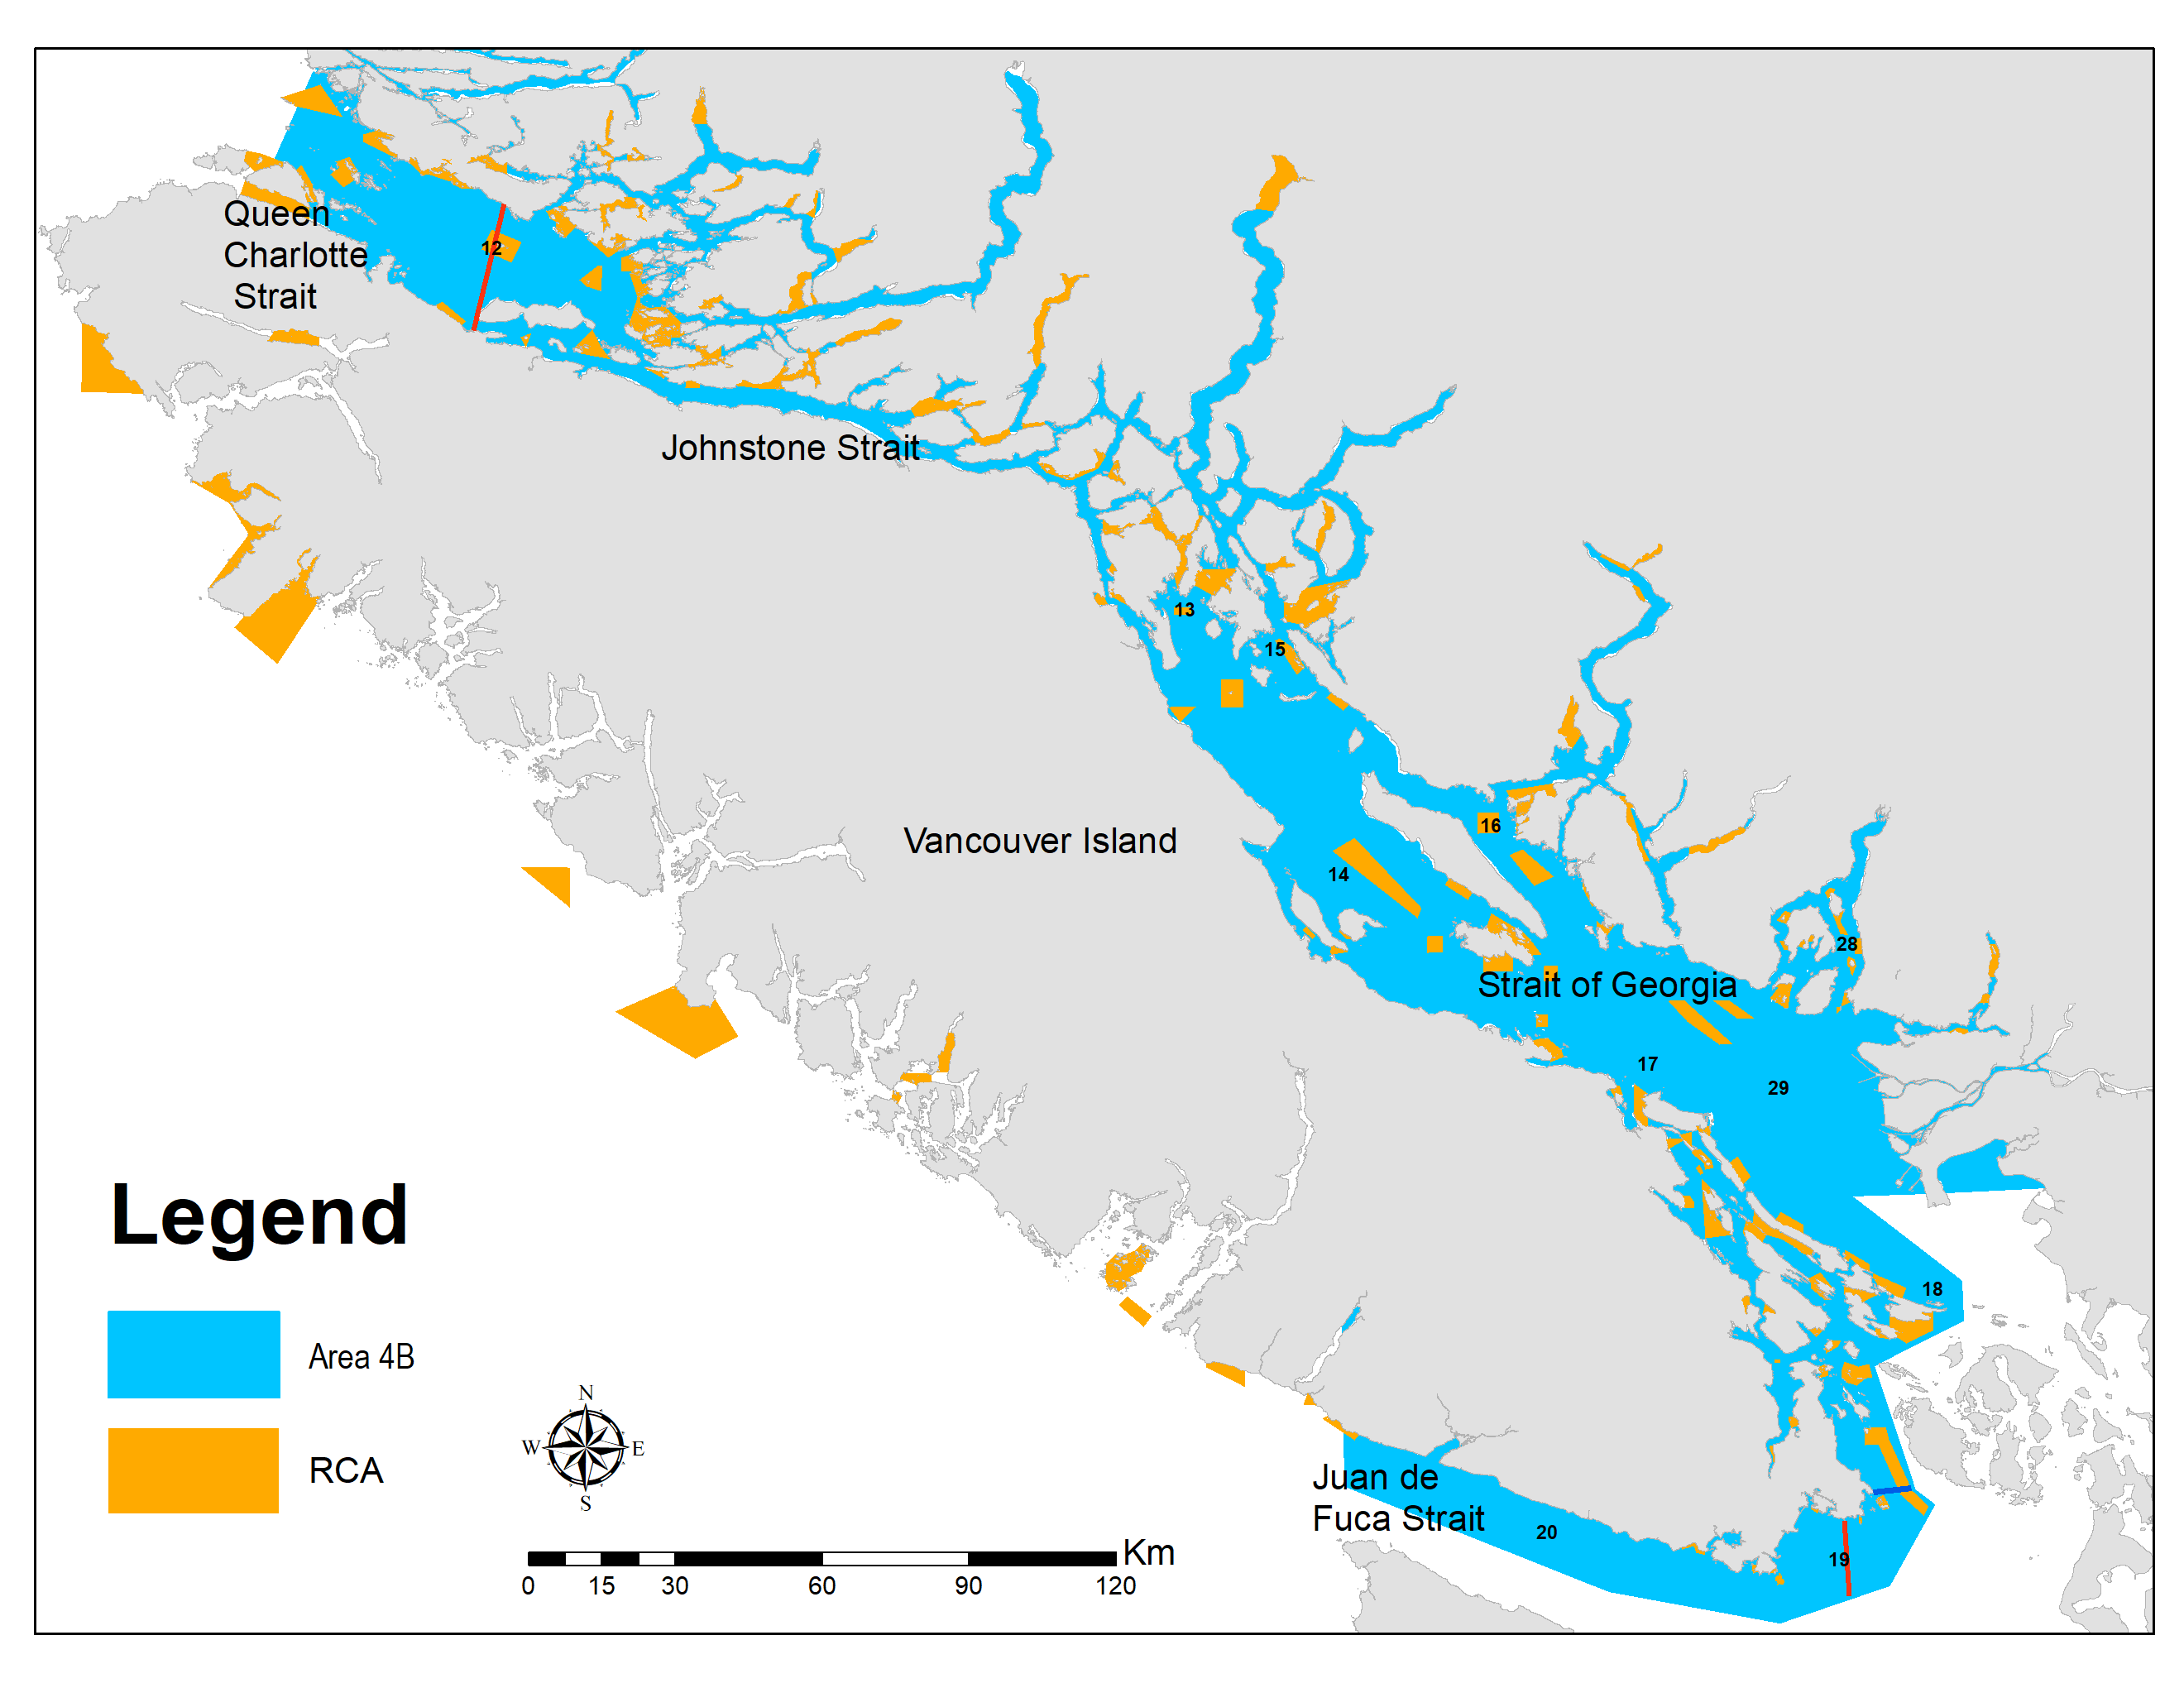
\includegraphics[width=5in]{C:/GitHub/yelloweye-inside/figs-french/InsideYE_Map_new}}{Figure \ref{fig:map-4B}} 

}

\caption{Carte de la zone de gestion 4B du poisson de fond montrant les aires de conservation du sébaste (ACS) et les limites séparant l'unité désignable (UD) du sébaste aux yeux jaunes des eaux intérieures de l'UD du sébaste aux yeux jaunes des eaux extérieures. Les lignes rouges indiquent une proposition d'ajustement de l'aire de répartition de l'UD des eaux intérieures, fondée sur des preuves génétiques récentes (Siegle \protect\hyperlink{ref-siegle2011}{2011}; Siegle et al. \protect\hyperlink{ref-siegle2013}{2013}; Andrews et al. \protect\hyperlink{ref-andrews2018}{2018}).}\label{fig:map-4B}
\end{figure}
L'objectif du plan de rétablissement actuel est de « reconstituer le stock au-dessus du PRL sur 80 ans avec une probabilité de réussite de 56 \% ». Le jalon cible est de « dégager des tendances positives au cours de chaque période de 10 ans ». La procédure de gestion actuelle du sébaste aux yeux jaunes des eaux intérieures vise à maintenir les prises annuelles totales (commerciales, récréatives, alimentaires, sociales et rituelles des Premières Nations et de relevé) à moins de 15 tonnes (voir l'annexe 9 du document DFO (\protect\hyperlink{ref-ifmp2018}{2018}) pour plus de renseignements).

D'après les directives, les plans de rétablissement au Canada doivent présenter une forte probabilité de rétablissement des stocks de poissons hors de la zone critique dans le délai prescrit (DFO \protect\hyperlink{ref-dfo2013}{2013}). Ce projet vise notamment à répondre à une préoccupation exprimée par les gestionnaires des pêches, à savoir que la probabilité de réussite de 56 \% énoncée dans le plan de rétablissement actuel (DFO \protect\hyperlink{ref-ifmp2018}{2018}) ne correspond pas à la définition d'une probabilité élevée.

Le document d'orientation indique également certaines mesures de gestion recommandées, comme le maintien des prélèvements par toutes les sources au niveau le plus bas possible, l'élaboration d'une règle de contrôle des prises et l'application de l'évaluation de la stratégie de gestion pour évaluer, par simulation, le rendement d'autres mesures de gestion pour atteindre les objectifs de rétablissement du stock (DFO \protect\hyperlink{ref-dfo2013}{2013}). Le plan de rétablissement actuel met en œuvre un total autorisé des captures annuel fixe de 15 tonnes (DFO \protect\hyperlink{ref-ifmp2018}{2018}), qui n'a pas été mis à l'essai par simulation.

Le sébaste aux yeux jaunes est une espèce qui vit longtemps (jusqu'à 121 ans en Colombie-Britannique, Keppel et Olsen \protect\hyperlink{ref-keppel2019}{2019}), dans des habitats démersaux rocheux répartis de manière irrégulière et discontinue sur la côte intérieure de la Colombie-Britannique (Yamanaka et al. \protect\hyperlink{ref-yamanaka2011}{2011}). Ces caractéristiques du cycle biologique rendent l'espèce vulnérable à la surexploitation par la pêche. Le stock des eaux intérieures est considéré comme étant à données limitées, car peu de données sont accessibles sur la composition selon l'âge, on manque de données biologiques sur les pêches commerciales, récréatives et des Premières Nations, et une incertitude entoure l'ampleur des prises historiques.

\hypertarget{sec:introduction-mse}{%
\subsection{ÉVALUATION DE LA STRATÉGIE DE GESTION}\label{sec:introduction-mse}}

À l'échelle mondiale, la fourniture d'avis scientifiques pour la gestion des pêches a évolué vers des approches axées sur l'évaluation de la stratégie de gestion (ou axées sur la gestion) (p.~ex., Butterworth et Punt \protect\hyperlink{ref-butterworth1999}{1999}; Rademeyer et al. \protect\hyperlink{ref-rademeyer2007}{2007}; Berkson et Thorson \protect\hyperlink{ref-berkson2015}{2015}; Geromont et Butterworth \protect\hyperlink{ref-geromont2015}{2015}; Carruthers et al. \protect\hyperlink{ref-carruthers2016}{2016}; Punt et al. \protect\hyperlink{ref-punt2016}{2016}). L'évaluation de la stratégie de gestion se concentre sur la détermination des procédures de gestion qui donnent les meilleurs résultats en ce qui concerne l'atteinte des objectifs convenus en matière de politique et de pêche, lorsqu'ils sont mis en œuvre dans un environnement de simulation en « boucle fermée » (figure~\ref{fig:mse-chart-basic}). Dans les pêches à production contrôlée, comme la pêche du poisson de fond en Colombie-Britannique, où les quotas sont gérés, les procédures de gestion décrivent les mesures de gestion pour l'établissement des limites des prises. Les données exigées dans les procédures de gestion peuvent varier considérablement, allant d'approches très riches en données, y compris les évaluations statistiques des prises selon l'âge avec des règles de contrôle des prises, à des règles de données simples (approches « limitées en données »), qui ne reposent que sur les données sur les prises et un indice de l'abondance (p.~ex., Geromont et Butterworth \protect\hyperlink{ref-geromont2015}{2015}; Carruthers et al. \protect\hyperlink{ref-carruthers2016}{2016}).

La simulation en boucle fermée diffère des approches d'évaluation classique des stocks parce qu'elle simule la rétroaction entre la mise en œuvre des procédures de gestion et le système sous-jacent (le stock de poisson et son environnement), décrite par un ou plusieurs modèles opérationnels. L'approche de la simulation en boucle fermée tient compte de l'effet des procédures de gestion sur le système, ainsi que des données futures recueillies dans le système et de leur utilisation chez les procédures de gestion (Punt et al. \protect\hyperlink{ref-punt2016}{2016}; Carruthers et Hordyk \protect\hyperlink{ref-carruthers2018}{2018}\protect\hyperlink{ref-carruthers2018}{a}; Anderson et al. \protect\hyperlink{ref-anderson2020gfmp}{2020}\protect\hyperlink{ref-anderson2020gfmp}{a}).


\begin{figure}[htb]

{\centering \pdftooltip{\includegraphics[width=6.3in]{C:/GitHub/yelloweye-inside/figs-french/mse-chart-simple2}}{Figure \ref{fig:mse-chart-basic}} 

}

\caption{Illustration du processus de simulation en boucle fermée des pêches d'après Anderson et al. (\protect\hyperlink{ref-anderson2020gfmp}{2020}\protect\hyperlink{ref-anderson2020gfmp}{a}), selon Punt et al. (\protect\hyperlink{ref-punt2016}{2016}). La procédure de gestion peut être fondée sur une règle de données simple (p.~ex., réduire les prises autorisées de x \% si l'indice du relevé diminue de y \%) ou peut être un modèle d'estimation combiné à une règle de contrôle des prises.}\label{fig:mse-chart-basic}
\end{figure}
\hypertarget{sec:introduction-approach}{%
\subsection{APPROCHE}\label{sec:introduction-approach}}

En raison des données limitées sur le stock de sébaste aux yeux jaunes des eaux intérieures, il est difficile d'évaluer le rendement prévu des mesures de gestion nécessaires pour rendre le stock conforme aux dispositions sur les stocks de poissons, c.-à-d.~pour le faire sortir de la zone critique dans le délai convenu et avec la probabilité convenue. La simulation-mise à l'essai en boucle fermée des procédures de gestion à données limitées permet d'évaluer le rendement relatif des procédures de gestion dans un éventail d'incertitudes entourant, par exemple, la biologie sous-jacente des poissons, l'erreur d'observation, l'erreur d'estimation et l'erreur de mise en œuvre (p.~ex., Kell et al. \protect\hyperlink{ref-kell2006}{2006}; Carruthers et al. \protect\hyperlink{ref-carruthers2016}{2016}).

Depuis 2017, une entente de partenariat entre l'Université de la Colombie-Britannique et le MPO (DFO \protect\hyperlink{ref-dfo_dlmtool_2017}{2017}) a facilité l'élaboration de deux progiciels à accès libre pour l'évaluation de la stratégie de gestion, mis en œuvre dans l'environnement de programmation statistique R (R Core Team \protect\hyperlink{ref-r2019}{2019})~: l'outil pour les méthodes à données limitées (DLMtool) (Carruthers et Hordyk \protect\hyperlink{ref-carruthers2018}{2018}\protect\hyperlink{ref-carruthers2018}{a}, \protect\hyperlink{ref-carruthers_hordyk_2018}{2018}\protect\hyperlink{ref-carruthers_hordyk_2018}{b}) et l'outil pour l'évaluation de la stratégie de gestion (MSEtool) (Huynh et al. \protect\hyperlink{ref-huynh_msetool_2019}{2019}). Après plusieurs années de développement, ces progiciels sont parmi les logiciels les plus rapides, les plus souples et les plus extensibles pour évaluer les stratégies de gestion des pêches. Ils peuvent être appliqués à des stocks pauvres ou riches en données, permettant d'évaluer rapidement plusieurs procédures de gestion en fonction d'objectifs de conservation et de pêche personnalisables, et d'évaluer les principaux compromis.

\hypertarget{sec:introduction-mp-framework}{%
\subsubsection{Cadre des procédures de gestion du poisson de fond en Colombie-Britannique}\label{sec:introduction-mp-framework}}

Le Cadre des procédures de gestion pour le poisson de fond en Colombie-Britannique (Anderson et al. \protect\hyperlink{ref-anderson2020gfmp}{2020}\protect\hyperlink{ref-anderson2020gfmp}{a}) a été élaboré parallèlement au présent document pour évaluer le rendement d'un large éventail de procédures de gestion pour les espèces de poisson de fond à données limitées. Le Cadre des procédures de gestion fait largement appel aux fonctions de DLMtool et de MSEtool, avec l'appui d'un progiciel R gfdlm (Anderson et al. \protect\hyperlink{ref-gfdlm}{2020}\protect\hyperlink{ref-gfdlm}{c}) rédigé par les auteurs de Anderson et al. (\protect\hyperlink{ref-anderson2020gfmp}{2020}\protect\hyperlink{ref-anderson2020gfmp}{a}), qui contient un ensemble d'outils de soutien logiciel et des visualisations personnalisées.

Nous suivons le Cadre des procédures de gestion pour sélectionner les procédures de gestion afin d'établir des limites des prises pour les stocks de poissons de fond à données limitées (Anderson et al. \protect\hyperlink{ref-anderson2020gfmp}{2020}\protect\hyperlink{ref-anderson2020gfmp}{a}). Notre évaluation du plan de rétablissement du sébaste aux yeux jaunes des eaux intérieures constitue la première application du Cadre des procédures de gestion pour produire un avis scientifique à l'appui des décisions sur les prises. Le cadre suit six étapes de pratiques exemplaires décrites ci-après et plus en détail dans Anderson et al. (\protect\hyperlink{ref-anderson2020gfmp}{2020}\protect\hyperlink{ref-anderson2020gfmp}{a}).

Les étapes des pratiques exemplaires sont fondées sur un examen effectué par Punt et al. (\protect\hyperlink{ref-punt2016}{2016}), qui a cerné cinq étapes clés du processus d'évaluation de la stratégie de gestion (étapes 2 à 6 ci-après). Une première étape supplémentaire du Cadre des procédures de gestion, qui définit le contexte décisionnel, a été définie par Gregory et al. (\protect\hyperlink{ref-gregory2012}{2012}) et Cox et Benson (\protect\hyperlink{ref-cox2016}{2016}). En grande partie, le logiciel DLMtool a été conçu pour permettre aux praticiens de suivre ces étapes (figure~\ref{fig:mse-chart}; Carruthers et Hordyk \protect\hyperlink{ref-carruthers2018}{2018}\protect\hyperlink{ref-carruthers2018}{a}).



Les six étapes sont les suivantes~:

Étape 1~: Définition du contexte décisionnel.

Étape 2~: Choix des objectifs et des paramètres de rendement.

Étape 3~: Choix des incertitudes/spécification des modèles opérationnels.

Étape 4~: Détermination des procédures de gestion possibles.

Étape 5~: Simulation de l'application des procédures de gestion.

Étape 6~: Présentation des résultats et choix de la procédure de gestion.

\clearpage
\begin{figure}[htb]

{\centering \pdftooltip{\includegraphics[width=\textwidth]{C:/GitHub/yelloweye-inside/figs-french/mse-chart}}{Figure \ref{fig:mse-chart}} 

}

\caption{Les étapes du processus d'évaluation de la stratégie de gestion selon Punt et al. (\protect\hyperlink{ref-punt2016}{2016}), tel que mis en œuvre dans DLMtool. Copié de Anderson et al. (\protect\hyperlink{ref-anderson2020gfmp}{2020}\protect\hyperlink{ref-anderson2020gfmp}{a}) et adapté de Carruthers et Hordyk (\protect\hyperlink{ref-carruthers2018}{2018}\protect\hyperlink{ref-carruthers2018}{a}). Cette figure complète la figure~\ref{fig:mse-chart-basic}.}\label{fig:mse-chart}
\end{figure}
Après la sélection et la mise en œuvre de la procédure de gestion pour l'établissement de la limite des prises (figure~\ref{fig:mse-chart}; par exemple, application de l'algorithme de la procédure de gestion sélectionnée à l'indice du relevé observé), la dernière étape nécessaire consiste à surveiller et à évaluer périodiquement le rendement de la procédure de gestion (DFO \protect\hyperlink{ref-dfo2013}{2013}; Dowling et al. \protect\hyperlink{ref-dowling2015a}{2015}; Carruthers et Hordyk \protect\hyperlink{ref-carruthers2018}{2018}\protect\hyperlink{ref-carruthers2018}{a}). Cela peut se faire par des moyens informels, comme à l'aide de la rétroaction des pêcheurs et des données des relevés (p.~ex., Cox et Kronlund \protect\hyperlink{ref-cox2008a}{2008}), ou au moyen de mesures statistiques plus formelles, où l'on compare les données observées aux prévisions des modèles opérationnels pour vérifier si le système fonctionne comme prévu (Butterworth \protect\hyperlink{ref-butterworth2008}{2008}; Carruthers et Hordyk \protect\hyperlink{ref-carruthers_hordyk_2018}{2018}\protect\hyperlink{ref-carruthers_hordyk_2018}{b}; discussion dans Anderson et al. \protect\hyperlink{ref-anderson2020gfmp}{2020}\protect\hyperlink{ref-anderson2020gfmp}{a}).

Dans les sections suivantes, nous décrivons notre approche pour l'élaboration d'un éventuel plan de rétablissement du sébaste aux yeux jaunes des eaux intérieures, en suivant les six étapes des pratiques exemplaires.

\hypertarget{sec:decision-context}{%
\section{DÉFINIR LE CONTEXTE DÉCISIONNEL}\label{sec:decision-context}}

Les principales questions qui guident la définition du contexte décisionnel de l'évaluation de la stratégie de gestion sont les suivantes~:

\emph{Quelle est la décision exacte à prendre? }Quel est le délai pour prendre la décision? \emph{Quels sont les rôles et responsabilités précis des parties concernées? Les parties sont les Sciences, la Gestion des pêches, les Premières Nations, l'industrie, le milieu universitaire et des organisations non gouvernementales. }Comment la décision finale sera-t-elle prise?

Pour ce plan de rétablissement, il faut décider de la procédure de gestion à utiliser pour déterminer les limites des prises pour la période allant jusqu'au prochain avis disponible sur les prises. Le Comité régional d'examen par les pairs devrait prendre la décision finale sur la procédure de gestion à appliquer pour déterminer les futures limites des prises sur une base consensuelle, après avoir examiné le contenu scientifique de l'avis (y compris la structure et le contenu des modèles opérationnels) et tenu compte du rendement relatif des procédures de gestion et des compromis entre les paramètres de rendement.

\hypertarget{sec:objectives-metrics}{%
\section{SÉLECTION DES OBJECTIFS ET DES PARAMÈTRES DE RENDEMENT}\label{sec:objectives-metrics}}

Il faut établir des objectifs clairs en matière de gestion et de pêche, ainsi que les paramètres de rendement qui permettent de les évaluer. Les objectifs peuvent couvrir un large éventail d'objectifs stratégiques ou législatifs (p.~ex., maintenir le stock au-dessus du PRL), d'objectifs économiques (p.~ex., maintenir des prises moyennes ou réduire la variabilité des prises) et d'objectifs culturels (p.~ex., maintenir l'accès minimal requis au stock ou à des zones de pêche particulières). Dans un scénario de rétablissement, les objectifs de conservation doivent avoir préséance. Cependant, dans un cadre de simulation, il est possible d'examiner des compromis entre la conservation et d'autres objectifs de pêche à court et à long terme, tant que l'objectif principal de conservation est atteint. Les objectifs entièrement quantifiés comprennent un paramètre ou une cible, la probabilité souhaitée de réussite et un délai pour atteindre l'objectif (p.~ex., la probabilité de maintenir le stock au-dessus du PRL est supérieure à 0,95 {[}19 fois sur 20{]} sur 1,5 génération du stock). Les paramètres de rendement sont des mesures quantifiées des objectifs. Dans une simulation en boucle fermée, ils sont calculés dans le modèle opérationnel à chaque étape temporelle des projections.

L'objectif initial du plan de rétablissement était de reconstituer le stock au-dessus du PRL sur 80 ans avec une probabilité de réussite de 56 \%. Un autre jalon cible était d'atteindre des tendances positives de la biomasse dans chaque période de 10 ans. La procédure de gestion convenue pour atteindre ces objectifs était de maintenir le TAC combiné (pêches commerciales, récréatives, ASR, de relevé biologique) à moins de 15 tonnes par année (DFO \protect\hyperlink{ref-ifmp2018}{2018}).

\hypertarget{sec:objectives-metrics-obj}{%
\subsection{OBJECTIFS ET JALONS}\label{sec:objectives-metrics-obj}}

Nous présentons un ensemble d'objectifs améliorés et les paramètres de rendement connexes pour le plan de rétablissement du sébaste aux yeux jaunes des eaux intérieures. Les principaux objectifs provisoires de conservation sont guidés par le Cadre de l'approche de précaution (DFO \protect\hyperlink{ref-dfo2006}{2006}, \protect\hyperlink{ref-dfo2009}{2009}), le document d'orientation du plan de rétablissement (DFO \protect\hyperlink{ref-dfo2013}{2013}) et les précédents régionaux (Cox et al. \protect\hyperlink{ref-cox2019}{2019}, \protect\hyperlink{ref-cox2020}{2020}). D'autres objectifs liés au rendement des pêches et à la variabilité du rendement annuel des pêches sont fondés sur des précédents dans d'autres analyses de la région du Pacifique du MPO (p.~ex., Cox et Kronlund \protect\hyperlink{ref-cox2008a}{2008}; Forrest et al. \protect\hyperlink{ref-forrest2018}{2018}; Cox et al. \protect\hyperlink{ref-cox2019}{2019}, \protect\hyperlink{ref-cox2020}{2020}).

L'objectif de conservation de base proposé est le suivant~:
\begin{enumerate}
\def\labelenumi{\arabic{enumi}.}

\item
  Ramener le stock au-dessus du PRL sur 56 ans (1,5 génération) avec une probabilité de réussite d'au moins 95 \% {[}19 fois sur 20{]}.
\end{enumerate}
Nous avons ajusté le délai de rétablissement initial de 80 ans (DFO \protect\hyperlink{ref-ifmp2018}{2018}) à 56 ans dans la présente analyse, en fonction de la durée de génération estimée pour le sébaste aux yeux jaunes des eaux extérieures (Cox et al. \protect\hyperlink{ref-cox2020}{2020}), en tenant compte de la directive selon laquelle le rétablissement doit être réalisé dans un délai de 1,5 à 2 durées de génération (DFO \protect\hyperlink{ref-dfo2013}{2013}). Pour de plus amples renseignements sur la durée de génération, consulter l'annexe~\ref{app:biological-data}, section~\ref{sec:generation}. Nous avons fait passer la probabilité de réussite souhaitée de 56 \% à 95 \% pour tenir compte de la directive selon laquelle la probabilité de rétablissement doit être élevée, ainsi que des pratiques exemplaires internationales, où les politiques de nombreuses administrations visent à maintenir les stocks au-dessus du PRL avec une probabilité de 90 \% à 95 \% {[}18 à 19 fois sur 20{]} (Sainsbury \protect\hyperlink{ref-sainsbury2008}{2008}; McIlgorm \protect\hyperlink{ref-mcilgorm2013}{2013}).

Nous proposons également les objectifs supplémentaires suivants, précisés dans la section~\ref{sec:objectives-metrics-pm}:
\begin{enumerate}
\def\labelenumi{\arabic{enumi}.}
\setcounter{enumi}{1}
\item
  Reconstituer le stock au-dessus du RSS sur 56 ans (1,5 génération).
\item
  Reconstituer le stock au-dessus du PRL sur 38 ans (1 génération).
\item
  Les objectifs de conservation ci-dessus étant atteints, maintenir des prises cibles moyennes à court et à long terme.
\item
  Les objectifs de conservation ci-dessus étant atteints, réduire au minimum la variabilité des prises dans les pêches d'une année à l'autre.
\end{enumerate}
Il convient de noter que nous n'avons pas attribué de probabilités cibles à ces objectifs, car elles sont fournies aux fins de l'évaluation des compromis avec l'objectif 1. Toutefois, nous avons éliminé les procédures de gestion qui ne respectaient pas la probabilité minimale de maintenir les prises au-dessus de 10 tonnes à court terme (voir la section~\ref{sec:simulation}).

En plus des objectifs susmentionnés, nous proposons de peaufiner les jalons définis dans le plan de rétablissement initial (DFO \protect\hyperlink{ref-ifmp2018}{2018}) en ajoutant le texte en italiques comme suit~:
\begin{enumerate}
\def\labelenumi{\arabic{enumi}.}
\setcounter{enumi}{5}

\item
  Atteindre des tendances positives de la biomasse dans chaque période de 10 ans \emph{tant que le stock demeure inférieur au PRL}.
\end{enumerate}
La période de 10 ans indiquée dans les jalons du plan de rétablissement actuel du sébaste aux yeux jaunes des eaux intérieures (DFO \protect\hyperlink{ref-ifmp2018}{2018}) reflétait une hypothèse selon laquelle le rétablissement hors de la zone critique pourrait être très lent pour ce stock. Nous avons ajusté le jalon pour tenir compte de l'hypothèse selon laquelle, une fois que le stock n'est plus dans la zone critique, le jalon ne sera plus nécessaire. La directive actuelle sur le rétablissement (DFO \protect\hyperlink{ref-dfo2013}{2013}) ne prévoit que des objectifs pour faire sortir les stocks de la zone critique, avec des jalons visant à garantir que les progrès sont réalisés pendant le processus de rétablissement. Elle mentionne des objectifs à plus long terme pour poursuivre le rétablissement des stocks jusque dans la zone saine, au-dessus du RSS. Toutefois, cela est censé se produire après la période du plan de rétablissement et en dehors de la portée de ce dernier (DFO \protect\hyperlink{ref-dfo2013}{2013}).

\hypertarget{sec:objectives-metrics-pm}{%
\subsection{PARAMÈTRES DE RENDEMENT}\label{sec:objectives-metrics-pm}}

Nous proposons les paramètres de rendement suivants pour mesurer les objectifs, où \emph{B} représente la biomasse féconde, RMD le rendement maximal durable, \emph{B}\textsubscript{RMD} la biomasse féconde à l'équilibre au rendement maximal durable, DG représente la durée d'une génération, et EAMP l'écart absolu moyen des prises (\(C\)) sur les \(n\) années (remarque~: \emph{CT} = court terme, \emph{LT} = long terme). Nous définissons le PRL et le RSS comme 0,4\emph{B}\textsubscript{RMD} et 0,8\emph{B}\textsubscript{RMD}, respectivement, en suivant les définitions provisoires du Cadre de l'approche de précaution (DFO \protect\hyperlink{ref-dfo2006}{2006}), utilisées dans l'évaluation des stocks de 2010 (Yamanaka et al. \protect\hyperlink{ref-yamanaka2011}{2011}). Dans les simulations en boucle fermée, tous les points de référence et les paramètres de rendement sont calculés dans le modèle opérationnel. Les paramètres de rendement bruts sont calculés pour chacune des 100 années de la période de projection et résumés en fonction de la période d'intérêt~: 1. \textbf{PRL 1,5DG}~: P(\emph{B} \textgreater{} 0,4 \emph{B}\textsubscript{RMD}) après 1,5 DG (en 2075, année 56 de la période de projection) 2. \textbf{RSS 1,5DG}~: P(\emph{B} \textgreater{} 0,8 \emph{B}\textsubscript{RMD}) après 1,5 DG (en 2075, année 56 de la période de projection) 3. \textbf{PRL 1DG}~: P(\emph{B} \textgreater{} 0,4 \emph{B}\textsubscript{RMD}) après 1 DG (en 2057, année 38 de la période de projection) 4. \textbf{CT C10}~: P(prises moyennes \textgreater{} 10 tonnes) de 2020 à 2029, années 1 à 10 de la période de projection 5. \textbf{CT C15}~: P(prises moyennes \textgreater{} 15 tonnes) de 2020 à 2029, années 1 à 10 de la période de projection 6. \textbf{LT C20}~: P(prises moyennes \textgreater{} 20 tonnes) après 1 DG (en 2057, année 38 de la période de projection) 7. \textbf{CT EAMP}~: P(EAMP\textsubscript{2020-2029} \textless{} EAMP\textsubscript{2012-2019})

Nous avons inclus le paramètre de rendement PRL 1 DG pour nous assurer que les procédures de gestion ne mènent pas le stock à l'effondrement à court terme. Nous avons choisi 10 tonnes, 15 tonnes et 20 tonnes comme cibles de prises, qui représentent des niveaux de prises de 5 tonnes inférieurs et supérieurs au TAC actuel de 15 tonnes.

Nous avons calculé EAMP\textsubscript{2020-2029} comme suit~:
\begin{equation}
\textrm{AADC}_\textrm{2020-2029} = \dfrac{1}{9}\sum_{y=2021}^{2029} \mid C_y - C_{y-1} \mid.
\end{equation}
Une période de référence (de 2012 à 2019) a été choisie, car elle marque le début du TAC de 15 tonnes. Nous avons calculé EAMP\textsubscript{2012-2019} comme suit~:
\begin{equation}
\textrm{AADC}_\textrm{2012-2019} = \dfrac{1}{7}\sum_{y=2013}^{2019} \mid C_y - C_{y-1} \mid.
\end{equation}
Lorsque les paramètres de rendement sont calculés sur plusieurs années, il faut prendre soin d'expliquer clairement la façon dont les statistiques sommaires sont calculées. Anderson et al. (\protect\hyperlink{ref-anderson2020gfmp}{2020}\protect\hyperlink{ref-anderson2020gfmp}{a}) suggéraient provisoirement de calculer les statistiques de rendement sur les répétitions et les années pour toute la période définie pour le paramètre de rendement. Nous suivons ce protocole. Par exemple, nous avons calculé la moyenne des paramètres des prises à court terme par rapport aux répétitions et aux années 2020 à 2029.

\hypertarget{environnement-informatique}{%
\section{ENVIRONNEMENT INFORMATIQUE}\label{environnement-informatique}}

Cette version du document a été produite sur 2021-11-17 17:18:16 avec R version 3.6.3 (2020-02-29) (R Core Team \protect\hyperlink{ref-r2019}{2019}) et des versions du progiciel R:
\begin{longtable}[]{@{}llll@{}}
\toprule
& Paquet & Version & Date \\
\midrule
\endhead
bookdown & bookdown & 0.24 & 2021-09-02 \\
cowplot & cowplot & 1.1.1 & 2020-12-30 \\
csasdown & csasdown & 0.0.10.9000 & 2021-08-13 \\
DLMtool & DLMtool & 5.4.3 & 2021-10-26 \\
dplyr & dplyr & 1.0.7 & 2021-06-18 \\
gfdata & gfdata & 0.0.0.9000 & 2021-07-05 \\
gfdlm & gfdlm & 0.0.1.9001 & 2021-10-26 \\
gfplot & gfplot & 0.1.4 & 2021-08-13 \\
ggplot2 & ggplot2 & 3.3.5 & 2021-06-25 \\
knitr & knitr & 1.36 & 2021-09-29 \\
MSEtool & MSEtool & 1.6.0 & 2020-05-05 \\
purrr & purrr & 0.3.4 & 2020-04-17 \\
rmarkdown & rmarkdown & 2.11 & 2021-09-14 \\
tidyr & tidyr & 1.1.4 & 2021-09-27 \\
TMB & TMB & 1.7.22 & 2021-09-28 \\
\bottomrule
\end{longtable}
\vspace{4mm}

\vspace{4mm}

Le code source de ce document est accessible à l'adresse suivante:\\
\url{https://github.com/pbs-assess/yelloweye-inside/tree/2f9a8a4}.

Ce document a été compilé avec le progiciel csasdown en R (Anderson et al. \protect\hyperlink{ref-csasdown}{2020}\protect\hyperlink{ref-csasdown}{b}).

Les versions particulières des logiciels de base utilisés pour générer ce rapport peuvent être consultées aux adresses:

\url{https://github.com/DLMtool/DLMtool/tree/fa971cf}\\
\url{https://github.com/tcarruth/MSEtool/tree/fa1498c}~\\
\url{https://github.com/pbs-assess/gfdata/tree/7292039}~\\
\url{https://github.com/pbs-assess/gfplot/tree/e0b36c0}~\\
\url{https://github.com/pbs-assess/gfdlm/tree/b895686}~\\
\url{https://github.com/pbs-assess/csasdown/tree/f9d5081}~\\

\clearpage

\hypertarget{refs}{}
\leavevmode\hypertarget{ref-anderson2020gfmp}{}%
Anderson, S.C., Forrest, R.E., Huynh, Q.C., et Keppel, E.A. 2020a. A management procedure framework for groundfish in British Columbia. DFO Can. Sci. Advis. Sec. Res. Doc. 2020/nnn: In prep.

\leavevmode\hypertarget{ref-csasdown}{}%
Anderson, S.C., Grandin, C., Edwards, A.M., Grinnell, M.H., Ricard, D., et Haigh, R. 2020b. csasdown: Reproducible CSAS Reports with bookdown. R package version 0.0.8.

\leavevmode\hypertarget{ref-gfdlm}{}%
Anderson, S.C., Grandin, C., et Forrest, R.E. 2020c. gfdlm: Tools for Working With DLMtool and MSEtool. R package version 0.0.1.9000. \url{https://github.com/pbs-assess/gfdlm}.

\leavevmode\hypertarget{ref-andrews2018}{}%
Andrews, K.S., Nichols, K.M., Elz, A., Tolimieri, N., Harvey, C.J., Pacunski, R., Lowry, D., Yamanaka, K.L., et Tonnes, D.M. 2018. Cooperative research sheds light on population structure and listing status of threatened and endangered rockfish species. Conserv. Genet. 19(4): 865‑878.

\leavevmode\hypertarget{ref-berkson2015}{}%
Berkson, J., et Thorson, J.T. 2015. The Determination of Data-Poor Catch Limits in the United States: Is There a Better Way? ICES J. Mar. Sci. 72(1): 237‑242.

\leavevmode\hypertarget{ref-butterworth2008}{}%
Butterworth, D.S. 2008. Some lessons from implementing management procedures. Edited by K. Tsukamoto, T. Kawamura, T. Takeuchi, T.D. Beard, Jr., and M.J. Kaiser. \emph{Dans} Fisheries for Global Welfare and Environment, 5th World Fisheries Congress 2008. TERRAPUB, Toyko. p. 381‑397.

\leavevmode\hypertarget{ref-butterworth1999}{}%
Butterworth, D.S., et Punt, A.E. 1999. Experiences in the Evaluation and Implementation of Management Procedures. ICES J. Mar. Sci. 56(6): 985‑998.

\leavevmode\hypertarget{ref-carruthers2018}{}%
Carruthers, T.R., et Hordyk, A. 2018a. The Data-Limited Methods Toolkit (DLMtool): An R package for informing management of data-limited populations. Methods Ecol. Evol. 9: 2388‑2395.

\leavevmode\hypertarget{ref-carruthers_hordyk_2018}{}%
Carruthers, T.R., et Hordyk, A.R. 2018b. Using management strategy evaluation to establish indicators of changing fisheries. Can. J. Fish. Aquat. Sci.: 1‑16.

\leavevmode\hypertarget{ref-carruthers2016}{}%
Carruthers, T.R., Kell, L.T., Butterworth, D.D.S., Maunder, M.N., Geromont, H.F., Walters, C., McAllister, M.K., Hillary, R., Levontin, P., Kitakado, T., et Davies, C.R. 2016. Performance Review of Simple Management Procedures. ICES J. Mar. Sci. J. Cons. 73(2): 464‑482.

\leavevmode\hypertarget{ref-cosewic2008}{}%
COSEWIC. 2008. COSEWIC assessment and status report on the Yelloweye Rockfish (\emph{Sebastes ruberrimus}), Pacific Ocean inside waters population and Pacific Ocean outside waters population, in Canada. Committee on the Status of Endangered Wildlife in Canada \url{https://www.sararegistry.gc.ca/virtual_sara/files/cosewic/sr_yelloweye_rockfish_0809_e.pdf}.

\leavevmode\hypertarget{ref-cox2016}{}%
Cox, S.P., et Benson, A.J. 2016. Roadmap to More Sustainable Pacific Herring Fisheries in Canada: A Step-by-Step Guide to the Management Strategy Evaluation Approach.

\leavevmode\hypertarget{ref-cox2019}{}%
Cox, S.P., Benson, A.J., Cleary, J.S., et Taylor, N.G. 2019. Candidate Limit Reference Points as a Basis for Choosing Among Alternative Harvest Control Rules for Pacific Herring (\emph{Clupea pallasii}) in British Columbia. DFO Can. Sci. Advis. Sec. Res. Doc. 2019/050. viii + 47 p.

\leavevmode\hypertarget{ref-cox2020}{}%
Cox, S.P., Doherty, B., Benson, A.J., Johnson, S.D., et Haggarty, D. 2020. Evaluation of potential rebuilding strategies for Outside Yelloweye Rockfish in British Columbia. DFO Can. Sci. Advis. Sec. Res. Doc. 2020/069. viii + 135 p.

\leavevmode\hypertarget{ref-cox2008a}{}%
Cox, S.P., et Kronlund, A.R. 2008. Practical Stakeholder-Driven Harvest Policies for Groundfish Fisheries in British Columbia, Canada. Fish. Res. 94(3): 224‑237.

\leavevmode\hypertarget{ref-dfo2006}{}%
DFO. 2006. A harvest strategy compliant with the Precautionary Approach. DFO Can. Sci. Advis. Sec. Sci. Advis. Rep. 2006/023.

\leavevmode\hypertarget{ref-dfo2009}{}%
DFO. 2009. A Fishery Decision-Making Framework Incorporating the Precautionary Approach \url{https://www.dfo-mpo.gc.ca/reports-rapports/regs/sff-cpd/precaution-back-fiche-eng.htm}.

\leavevmode\hypertarget{ref-dfo2012}{}%
DFO. 2012. Survey of Recreational Fishing in Canada 2010. DFO Res. Manage. Eco. Fish. Manage. 2012-1804.

\leavevmode\hypertarget{ref-dfo2013}{}%
DFO. 2013. Guidance for the development of rebuilding plans under the Precautionary Approach framework~: growing stocks out of the critical zone \url{https://www.dfo-mpo.gc.ca/reports-rapports/regs/sff-cpd/precautionary-precaution-eng.htm}.

\leavevmode\hypertarget{ref-dfo_dlmtool_2017}{}%
DFO. 2017. DLMtool Phase II: Developing a Management Strategy Evaluation Package for Advancing the Science and Management of Data-limited and at-risk Canadian Fish Stocks. PAC2016.12.

\leavevmode\hypertarget{ref-ifmp2018}{}%
DFO. 2018. Pacific Region integrated fisheries management plan, groundfish, effective February 21, 2018 \url{http://waves-vagues.dfo-mpo.gc.ca/Library/40657814.pdf}.

\leavevmode\hypertarget{ref-dowling2015a}{}%
Dowling, N.A., Dichmont, C.M., Haddon, M., Smith, D.C., Smith, A.D., et Sainsbury, K. 2015. Guidelines for Developing Formal Harvest Strategies for Data-Poor Species and Fisheries. Fish. Res. 171: 130‑140.

\leavevmode\hypertarget{ref-forrest2018}{}%
Forrest, R.E., Holt, K.R., et Kronlund, A.R. 2018. Performance of Alternative Harvest Control Rules for Two Pacific Groundfish Stocks with Uncertain Natural Mortality: Bias, Robustness and Trade-Offs. Fish. Res. 206: 259‑286.

\leavevmode\hypertarget{ref-geromont2015}{}%
Geromont, H.F., et Butterworth, D.S. 2015. Complex Assessments or Simple Management Procedures for Efficient Fisheries Management: A Comparative Study. ICES J. Mar. Sci. 72(1): 262‑274.

\leavevmode\hypertarget{ref-gregory2012}{}%
Gregory, R., Failing, L., Harstone, M., Long, G., et McDaniels, T.L. (\emph{Éditeurs}). 2012. Structured Decision Making: A Practical Guide to Environmental Management Choices. Wiley-Blackwell, Oxford.

\leavevmode\hypertarget{ref-huynh_msetool_2019}{}%
Huynh, Q.C., Hordyk, A.R., et Carruthers, T. 2019. MSEtool: Management Strategy Evaluation Toolkit. R package version 1.4.3.

\leavevmode\hypertarget{ref-kell2006}{}%
Kell, L.T., De Oliveira, J.A.A., Punt, A.E., McAllister, M.K., et Kuikka, S. 2006. Chapter 15 Operational Management Procedures: An Introduction to the Use of Evaluation Frameworks. Developments in Aquaculture and Fisheries Science 36: 379‑407.

\leavevmode\hypertarget{ref-keppel2019}{}%
Keppel, E.A., et Olsen, N. 2019. Pre-COSEWIC review of Yelloweye Rockfish (\emph{Sebastes ruberrimus}) along the Pacific Coast of Canada: biology, distribution and abundance trends. DFO Can. Sci. Advis. Sec. Res. Doc 2019/014.

\leavevmode\hypertarget{ref-mcilgorm2013}{}%
McIlgorm, A. 2013. Literature study and review of international best practice in fisheries harvest strategy policy approaches. A Report to the Department of Agriculture, Fisheries and Forestry (DAFF) Canberra, by the Australian National Centre for Ocean Resources and Security (ANCORS), University of Wollongong. Final Report, March 26, 2013.

\leavevmode\hypertarget{ref-punt2016}{}%
Punt, A.E., Butterworth, D.S., de Moor, C.L., De Oliveira, J.A.A., et Haddon, M. 2016. Management Strategy Evaluation: Best Practices. Fish Fish. 17(2): 303‑334.

\leavevmode\hypertarget{ref-rademeyer2007}{}%
Rademeyer, R.A., Plagányi, É.E., et Butterworth, D.S. 2007. Tips and Tricks in Designing Management Procedures. ICES J. Mar. Sci. 64(4): 618‑625.

\leavevmode\hypertarget{ref-r2019}{}%
R Core Team. 2019. R: A Language and Environment for Statistical Computing. R Foundation for Statistical Computing, Vienna, Austria.

\leavevmode\hypertarget{ref-sainsbury2008}{}%
Sainsbury, K. 2008. Best Practice Reference Points for Australian Fisheries. Report to the Australian Fisheries Management Authority.

\leavevmode\hypertarget{ref-siegle2011}{}%
Siegle, M.R. 2011. Population structure in yelloweye rockfish (\emph{Sebastes ruberrimus}) driven by limited dispersal and selection. Thesis.

\leavevmode\hypertarget{ref-siegle2013}{}%
Siegle, M.R., Taylor, E.B., Miller, K.M., Withler, R.E., et Yamanaka, K.L. 2013. Subtle Population Genetic Structure in Yelloweye Rockfish (\emph{Sebastes ruberrimus}) Is Consistent with a Major Oceanographic Division in British Columbia, Canada. PLoS ONE 8(8): e71083.

\leavevmode\hypertarget{ref-yamanaka2011}{}%
Yamanaka, K.L., McAllister, M.K., Olesiuk, P.F., Etienne, M.-P., Obradovich, S.G., et Haigh, R. 2011. Stock assessment for the inside population of Yelloweye Rockfish (\emph{Sebastes ruberrimus}) for British Columbia, Canada for 2010. DFO Can. Sci. Advis. Sec. Res. Doc. 2011/129. xiv + 131 p.

\end{document}
